\documentclass{FR16} 

\begin{document}

\maketitle

\newpage
\tableofcontents
\newpage
\section{Abstract}
The aim of the project is to analyse the data from the "New York City Airbnb Open Data" from the Kaggle website.
\\ In particular, we focus on the developing of predictive model to forecast the house' prices using Supervised Learning algorithms: 
\begin{itemize}
\item Decision Tree
\item Random Forest
\item Ranger Random Forest
\item Linear Regression
\item Neural Newtworks (?)
\end{itemize}
A crucial part of the project was to the tuning and finding of the hyperparameters of the different models in order to get the best fit.
%%Eachreport must contain:\\
%•shortabstract: what are your going to present %in the report\\
%•statementof the problem/goalof the analysis %and description of thedata set(s)\\
%•list of three to fivefindings/keypoints\\
%•the analysis with wisecommentary\\
%•(optional) theoretical background of the used %methods\\
%•conclusions(should include the findings/%keypoints)\\
%•theAppendix, containing all the R codeNotice:
%\\•Thepaper lengthisirrelevant provided that %the content is correct.
%\\•No R code in the main text.The R code must %be confined to the appendix\\
%•The report should be prepared inPDFonly

\newpage
\section{Goal}
The goal is developing different models in order to predict the price of a house in New York.
\newpage
\section{Discussion}


\subsection{Dataset }
The dataset used in this project is one of a Kaggle competiotion and is called the New York City Airbnb Open Data. It contains 48.000 data points for each different column.
The dataset has different columns: 
\begin{itemize}
\item id
\item \textbf{name}: name of the listing
\item \textbf{host\_id}
\item \textbf{host\_name}
\item \textbf{neighbourhood\_group}: location
\item \textbf{neighbourhood}: area
\item \textbf{latitude}: coordinates
\item \textbf{longitude}: coordinates
\item \textbf{room\_type}: space type
\item \textbf{price}:  in dollars
\item \textbf{minimum\_nights}: amount of nights minimum
\item \textbf{number\_of\_reviews}: number of reviews
\item \textbf{last\_review}: latest review
\item \textbf{reviews\_per\_month}: number of reviews per month
\item \textbf{calculated\_host\_listings\_count}: amount of listing per host
\item  \textbf{availability\_365}: number of days when listing is available for booking\\
\end{itemize}
We select just 5 of this feature from the dataset since we denotes them as the most important for the price of a house: latitude, longitude, room type, neighbourhood and the price itself to compare the prediction during the tests. \\
\begin{figure}[H]
\centering
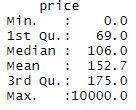
\includegraphics[width=0.3\textwidth]{figures/figure1.jpg} \\
\caption{\label{fig:1}Price summary}
\end{figure}
From the Figure 1 is possible to see that there are some outliers in the dataset that can not be removed, since we have to take in account that could be present luxury houses. In fact, no outlier was removed from the dataset. Also, there were no null and missing value apart from the reviews\_per\_month column that we do not take in account in the project.
\\ 
\subsection{Data Pre-processing}
The dataset has more or less 48.000 data points for each column, so an important part of this work was the pre-processing since it is large. Since the dataset is very large, running the different methods is time consuming. Scaling the numerical data is a key point to get better performance during the fitting process of the model.
We starting scaling numerical data from -1 to 1, using pre installed R functions while for the categorical data we identify each label with a different integer number.\\
The categorical features from the selected are: neighbourhood and room type.\\
The numerical features are: latitude, longitude and price.


\subsection{Decision Tree}
Decision  tree are one of the most used model in the Machine Learning world since are very familiar to human users and can be easily plotted. 
\\



\subsection{Random Forest}
Random Forest is an ensemble method which use a combination of decision tree to get the prediction.
\subsubsection{Ranger Random Forest}
Ranger Random Forest is a computationally light model which results are very close the classical Random Forest.
\\

\subsection{Linear Regression}



\newpage
\section{Results}
\subsection{Decision Tree}
\subsection{Random Forest results}
\subsection{Ranger Random Forest results}
\subsection{Linear Regression results}
\subsection{Neural Networks results}
\newpage
\section{Conclusion}
From the result the method with the most higher accuracy is the Random Forest method... while the worst are ....
\\Moreover, Random Forest method is also the worst in term of computation time for the tuning part since it takes for a configuration with 4 core, more or less 1 hour to tune the parameters. 


\newpage
\section{Appendix}

\newpage

\section{Tabelle e grafici}
Here a few examples of tables and graphs.
\subsection{Tabelle}
\begin{center}
\begin{tabular}{c c c c c c c c}
\arrayrulecolor{Azzurro}
\hline
{\bfseries $Codice$} & {\bfseries $CdL$} & {\bfseries $Lotto$} & {\bfseries $T_{setup/lotto}$} & {\bfseries $T_{lav/pezzo}$} & {\bfseries $T_{proc/pezzo}$} & {\bfseries$Quantit\grave{a}$} & {\bfseries $T_{tot}$}\\
\hline
100 & 4 & 250 & 25 & 0,5 & 0,6 & 1 & 0,6\\
111 & 2 & 250 & 20 & 2 & 2,08 & 1 & 2,08 \\
111 & 3 & 250 & 15 & 1,5 & 1,56 & 1 & 1,56 \\
112 & 2 & 250 & 20 & 2,5 & 2,58 & 1 & 2,58 \\
112 & 3 & 250 & 15 & 2 & 2,06 & 1 & 2,06\\
113 & 3 & 500 & 15 & 1 & 1,03 & 2 & 2,06\\
120 & 1 & 50 & 30 & 2 & 2,6 & 0,1 & 0,26\\
121 & 1 & 25 & 30 & 3 & 4,2 & 0,1 & 0,42 \\
121 & 1 & 25 & 30 & 2,5 & 3,7 & 0,1 & 0,37 \\
\hline
\end{tabular}
\end{center}

\subsubsection{Altra tabella}
\subsection{Grafici}
\begin{center}

\end{center}



\section{Altro}
\begin{figure}[H]
\centering
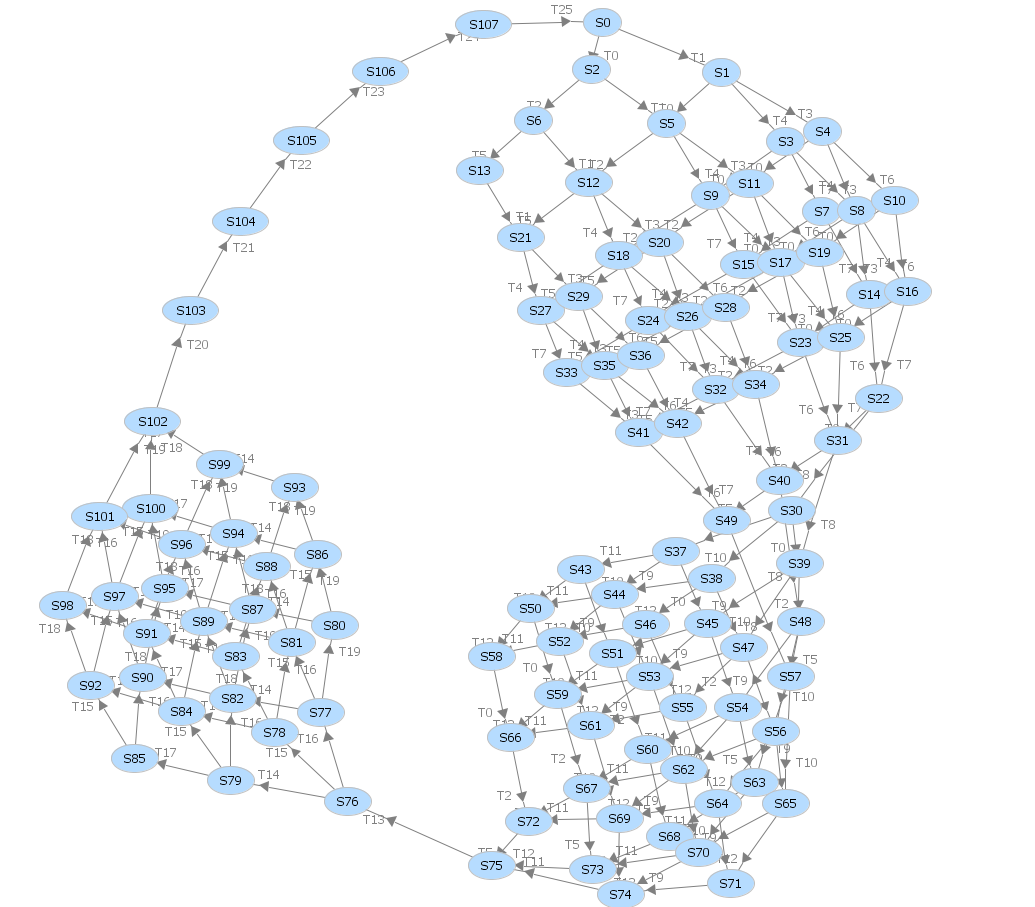
\includegraphics[width=1\textwidth]{grafo.png}
\caption{\label{fig:1}Didascalia.}
\end{figure}
\subsection{Footnote}
You can create a footnote like this.\footnote{I created a footnote.}



\newpage
\begin{thebibliography}{9}
\bibitem{giusti}
Giusti, Santochi, \emph{Tecnologia Meccanica e Studi di Fabbricazione}. Casa Editrice Ambrosiana, Seconda Edizione
\bibitem{mechteacher}
Mechteacher, \emph{Knuckle Joint – Introduction, Parts and Applications},\\ http://mechteacher.com/knuckle-joint/
\bibitem{totalmateria}
Totalmateria, \emph{G32NiCrMo8}, http://www.totalmateria.com 
\bibitem{sandvik}
Sandvik Coromant,\emph{Catalogo  generale  2018},   http://www.coromant.sandvik.com/it
\bibitem{uni}
Norme UNI, Ente nazionale italiano di unificazione
\end{thebibliography}

\end{document}